\documentclass[english]{beamer}\usepackage[]{graphicx}\usepackage[]{xcolor}
% maxwidth is the original width if it is less than linewidth
% otherwise use linewidth (to make sure the graphics do not exceed the margin)
\makeatletter
\def\maxwidth{ %
  \ifdim\Gin@nat@width>\linewidth
    \linewidth
  \else
    \Gin@nat@width
  \fi
}
\makeatother

\definecolor{fgcolor}{rgb}{0.345, 0.345, 0.345}
\newcommand{\hlnum}[1]{\textcolor[rgb]{0.686,0.059,0.569}{#1}}%
\newcommand{\hlstr}[1]{\textcolor[rgb]{0.192,0.494,0.8}{#1}}%
\newcommand{\hlcom}[1]{\textcolor[rgb]{0.678,0.584,0.686}{\textit{#1}}}%
\newcommand{\hlopt}[1]{\textcolor[rgb]{0,0,0}{#1}}%
\newcommand{\hlstd}[1]{\textcolor[rgb]{0.345,0.345,0.345}{#1}}%
\newcommand{\hlkwa}[1]{\textcolor[rgb]{0.161,0.373,0.58}{\textbf{#1}}}%
\newcommand{\hlkwb}[1]{\textcolor[rgb]{0.69,0.353,0.396}{#1}}%
\newcommand{\hlkwc}[1]{\textcolor[rgb]{0.333,0.667,0.333}{#1}}%
\newcommand{\hlkwd}[1]{\textcolor[rgb]{0.737,0.353,0.396}{\textbf{#1}}}%
\let\hlipl\hlkwb

\usepackage{framed}
\makeatletter
\newenvironment{kframe}{%
 \def\at@end@of@kframe{}%
 \ifinner\ifhmode%
  \def\at@end@of@kframe{\end{minipage}}%
  \begin{minipage}{\columnwidth}%
 \fi\fi%
 \def\FrameCommand##1{\hskip\@totalleftmargin \hskip-\fboxsep
 \colorbox{shadecolor}{##1}\hskip-\fboxsep
     % There is no \\@totalrightmargin, so:
     \hskip-\linewidth \hskip-\@totalleftmargin \hskip\columnwidth}%
 \MakeFramed {\advance\hsize-\width
   \@totalleftmargin\z@ \linewidth\hsize
   \@setminipage}}%
 {\par\unskip\endMakeFramed%
 \at@end@of@kframe}
\makeatother

\definecolor{shadecolor}{rgb}{.97, .97, .97}
\definecolor{messagecolor}{rgb}{0, 0, 0}
\definecolor{warningcolor}{rgb}{1, 0, 1}
\definecolor{errorcolor}{rgb}{1, 0, 0}
\newenvironment{knitrout}{}{} % an empty environment to be redefined in TeX

\usepackage{alltt}

%% The most common packages are already included in:
\usetheme{biostat}
%%%%%%%%%%%%%%%%%%%%%%%%%%%%%%%%%%%%%%%%%%%%%%%%%%%%%%%% 

%% Header data: (adjust to your needs:
\def\uzhunit{Biostatistics}             %% if (not) needed comment/uncomment
%\def\uzhunitext{STA480}

\title[Multicollinearity]{Multicollinearity}
%% Optional Argument in [Brackets]: Short Title for Footline

%% The following are all optional, simply comment them
%\subtitle{Subtitle (optional)}
%\institute{Biostatistics Journal Club}  %% optional
\author{Jerome Sepin}
%\date{\today}
%%%%%%%%%%%%%%%%%%%%%%%%%%%%%%%%%%%%%%%%%%%%%%%%%%%%%%%% 



%%%%%%%%%%%%%%%%%%%%%%%%%%%%%%%%%%%%%%%%%%%%%%%%%%%%%%%% 
\IfFileExists{upquote.sty}{\usepackage{upquote}}{}
\begin{document}
\maketitle
%%%%%%%%%%%%%%%%%%%%%%%%%%%%%%%%%%%%%%%%%%%%%%%%%%%%%%

%===================================================
\begin{frame}{Why this presentation?}
%===================================================
From \cite{Schwabe2022}:

\textit{
"The primary pharmacokinetic parameters were log-transformed and analyzed using an analysis of covariance (ANCOVA) model that included treatment as a fixed effect, \colorbox{yellow}{baseline weight} category $\left(\geq 60-\leq 80kg/>80\text{kg}-\leq 100\text{kg}\right)$, \colorbox{yellow}{baseline BMI} (continuous variable), and study site as covariates." 
}
\begin{center}
$\boxed{\log(y)\sim trt + weight_{cat.} + BMI_{cont.}+ site}$
\end{center}

%===================================================
\end{frame}
\begin{frame}{What is the problem with this?}
%===================================================
\begin{center}
$\boxed{\log(y)\sim trt + weight_{cat.} + BMI_{cont.}+ site}$
\end{center}
Since $\text{BMI}=\frac{\text{weight (kg)}}{\text{height (m)}^2}$
\begin{center}
$\boxed{\log(y)\sim trt + weight_{cat.} + \frac{weight_{cont.}}{height^2_{cont.}}+ site}$
\end{center}

Thus, $weight$ and $BMI$ may be highly correlated (a special case of collinearity)!




%===================================================
\end{frame}
\begin{frame}{What is the problem with collinear variables in the model?}
%===================================================

Let's see what happens when the correlation between $height$ and $weight$ changes!

\begin{figure}[h]%H is strict!
\begin{center}
\begin{knitrout}
\definecolor{shadecolor}{rgb}{0.969, 0.969, 0.969}\color{fgcolor}
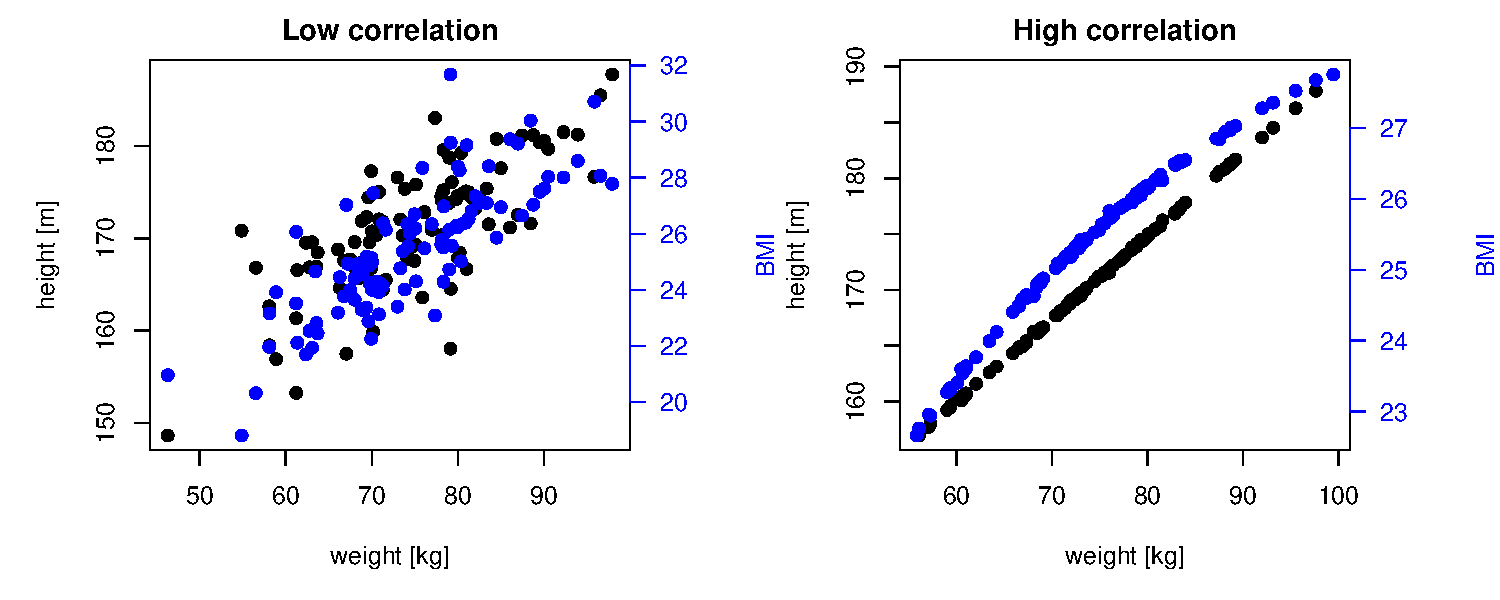
\includegraphics[width=\maxwidth]{figures/figcollinearitydata-1} 
\end{knitrout}
\end{center}
\end{figure}

%===================================================
\end{frame}
\begin{frame}{Small simulation:}
%===================================================

\begin{center}
$\boxed{\log(y)\sim trt + weight_{cat.} + BMI_{cont.}+ site}$

For simplicity without $site$ and with continuous variables!

"True" model: $\log(y)\sim 5 + 5\cdot trt + 2\cdot weight + 2\cdot height$





\textcolor{red}{Dichotomia is a problem for a different day\dots}
\end{center}


% %===================================================
% \end{frame}
% \begin{frame}{Relation of variables}
% %===================================================
% \begin{enumerate}
% \item paper: $AUC\sim trt + weight_{cat.} + BMI_{cont.}\textcolor{gray}{+ site}$
% 
% $AUC\sim trt + weight_{cat.} + \frac{weight_{cont.}}{height_{cont.}^2}\textcolor{gray}{+ site}$
% \item a1: $AUC\sim trt + weight_{cat.} + height_{cont.}\textcolor{gray}{+ site}$
% \item a2: $AUC\sim trt + weight_{cont.} + height_{cont.}\textcolor{gray}{+ site}$
% \end{enumerate}
% 
% Let's see what happens when the correlation between $height$ and $weight$ changes!

%===================================================
\end{frame}
\begin{frame}[plain]{Small simulation: Results}
%===================================================

\begin{figure}[h]%H is strict!
\begin{center}
\begin{knitrout}
\definecolor{shadecolor}{rgb}{0.969, 0.969, 0.969}\color{fgcolor}
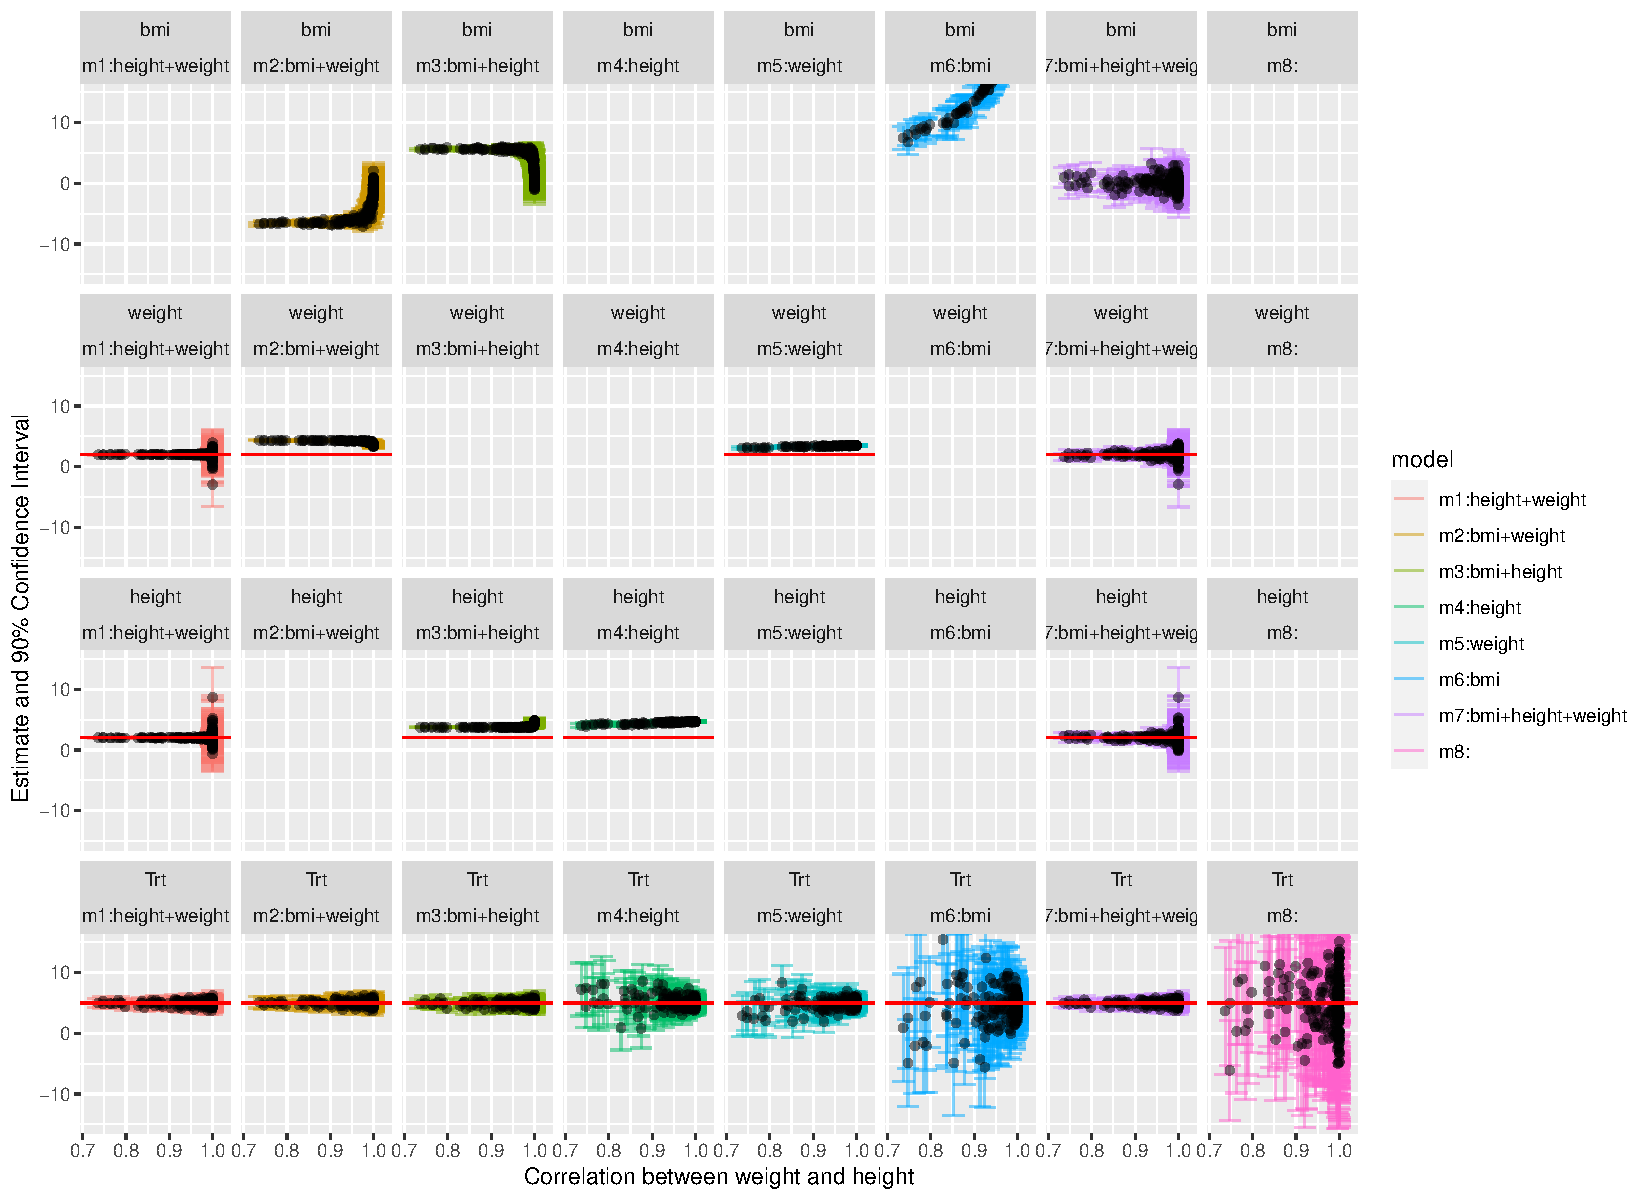
\includegraphics[width=\maxwidth]{figures/figresults-1} 
\end{knitrout}
\end{center}
\end{figure}

%===================================================
\end{frame}
\begin{frame}{Relation of variables}
%===================================================

\tikzstyle{block} = [draw=black, thick, text width=2cm, minimum height=1cm, align=center]
\tikzstyle{cloud} = [draw=black, ellipse, text width=1cm, minimum height=1cm, align=center] 
% \tikzstyle{cloud} = [draw, ellipse,fill=red!20, node distance=3cm,
%     minimum height=2em]
\tikzstyle{arrow} = [thick,->,>=stealth]

\begin{figure}[H]
\centering
\resizebox{8.5cm}{!}{%
\begin{tikzpicture}
		\node[cloud] (T) {T};
    \node[cloud,below right=3cm and 3cm of T] (weight) {$\textit{weight}_0$};
    \node[cloud, right=1.5cm of weight] (height) {$\textit{height}_0$};
    \node[cloud, below right=1.5cm and 4.5cm of T] (BMI) {$\textit{BMI}_0$};
		\node[cloud, right=9cm of T] (Y) {$Y$};

    % edges
    \draw[red] (T) -- (Y);
    \draw[line width=1.5mm ] (weight) -- (BMI);
    \draw[line width=1.5mm ] (height) -- (BMI);
    \draw (height) -- (weight);
    \draw (height) -- (Y);
    \draw (BMI) -- (Y);
    \draw (weight) to [bend right=80] (Y);
    \draw[gray!10] (BMI) -- (T);
    \draw[gray!10] (weight) -- (T);
    \draw[gray!10] (height) to [bend left=80] (T);

\end{tikzpicture}
}
\vspace*{-1.5cm}
\caption{Successful randomization removes confounding}
\end{figure}
\vspace*{-0.8cm}
\begin{center}
$\boxed{\text{BMI}=\frac{\text{weight (kg)}}{\text{height (m)}^2}}$
\end{center}

%===================================================
\end{frame}
\begin{frame}{But why this model?}
%===================================================
\centering
\huge{\textbf{Domain knowledge?}}

%===================================================
\end{frame}
\begin{frame}[plain]{But why this model?}
%===================================================
ICH E9:
\textit{
\tiny{
"In multicentre trials (see Glossary) the randomisation procedures should be organised centrally. It is advisable to have a separate random scheme for each centre, i.e. to stratify by centre or to allocate several whole blocks to each centre. More generally, stratification by important prognostic factors measured at baseline (e.g. severity of disease, age, sex, etc.) may sometimes be valuable in order to promote balanced allocation within strata; this has greater potential benefit in small trials. The use of more than two or three stratification factors is rarely necessary, is less successful at achieving balance and is logistically troublesome. The use of a dynamic allocation procedure (see below) may help to achieve balance across a number of stratification factors simultaneously provided the rest of the trial procedures can be adjusted to accommodate an approach of this type.}\footnotesize{
\cbox{Factors on which randomisation has been stratified should be accounted for later in the analysis.}"
}
}

%===================================================
\end{frame}
\begin{frame}{Collinearity != Correlation}
%===================================================

\begin{itemize}
\item Correlation is a special case of collinearity (includes only two variables)
\item Problems can also arise without large (pairwise) correlations
\item For example when explanatory variables add up to 100\% (recipe)
\end{itemize}


\begin{table}[]
\centering
%\resizebox{\textwidth}{!}{%
\begin{tabular}{|l|l|l|l|}
\hline
milk & water & ... & salt \\ 
\hline
40\% & 30\%  & ... & 1\%  \\ 
45\% & 35\%  & ... & 2\%  \\
\dots& \dots  & \dots & \dots  \\ \hline
\end{tabular}%
%}
\end{table}




%===================================================
\end{frame}
\begin{frame}{ }
%===================================================
Recipes remain secret!
\centering
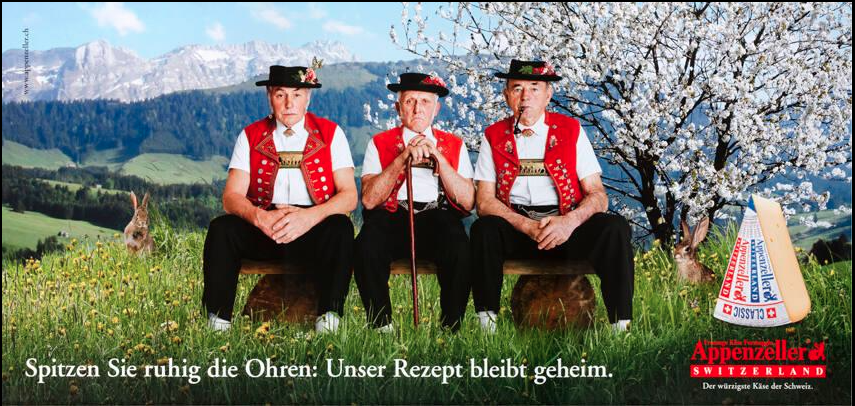
\includegraphics[width=0.9\textwidth]{appenzeller.png}

%===================================================
\end{frame}
\begin{frame}{Conclusion}
%===================================================

\begin{itemize}
\item Collinearity increases uncertainty (but only for the variables that contribute)
\item "Avoiding" collinearity may induce bias
\item Randomization to the help
\end{itemize}


%===================================================
\end{frame}
\begin{frame}{References}
%===================================================
  \small
  \bibliographystyle{apalike}
\bibliography{illustration}

\end{frame}

%\appendix
%% Possible backup slides...

%% chapter division is accomplished with:
%% \part{Appendix}

\end{document}
